\chapter{基于注意力机制的局部对齐网络}

\section{引言}
基于深度学习的服装检索网络一般可以概括为两个子网络:表示和匹配。表示网络即特征提取器,一般使用在ImageNet预训练的主流深度卷积网络,比如VGG、ResNet等主流骨干网络;
匹配网络对所提取特征进一步学习,以获得更适合服装检索这个任务的特征。特征提取器输出的特征经过Pooling之后得到一个向量之后,一般都会引入度量学习去做监督,
使同款的服装特征相似度提高,不同款的服装特征相似度降低,特征的相似度或者距离衡量常用余弦相似度。
常用的度量学习损失有Contrastive loss\cite{hadsell2006dimensionality}、Triplet loss\cite{schroff2015facenet}等。

大家在早期对服装检索的研究主要关注在全局信息上,即对整幅图提取一个全局的特征,但是后来这种方式遇到了瓶颈,大家开始慢慢把研究的方向转向对局部特征的学习与表示。
对于服装图像来说,全局信息包含了更加丰富的语义信息,但是对局部信息的抽取也非常有帮助,因为不同款式的服装有的时候仅仅有着细微的差别,在全局特征中,这些重要
但是不明显或者所占区域比例较小的局部信息会被Average Pooling稀释掉,如果可以通过某种方式将这个区域的特征单独提取出来,或者强化这个局部区域的特征强度,
对检索结果将会带来巨大的收益。比较常用的局部特征提取方法有对输入图像的切分\cite{varior2016siamese},或者网格\cite{li2014deepreid}等,这种方式直接获取局部特征
比较简单直接,但是也有其相应的不足之处:同款服装的不同拍摄图像摆放位置及形状不一定相同,两幅图的局部特征并不能很好的对齐。
Fashion-Net使用关键点信息协助局部的定位,网络第一阶段先生成对关键点位置的预测,第二阶段根据关键点位置对局部信息Pooling。通过关键点的方式可以很好的解决局部部件对齐
的问题,但是这个方法需要训练样本有对应关键点的标注信息,带来的资源消耗较大。

近年来,注意力机制(Attention Mechanism)在深度学习的各个领域都被广泛的使用,从自然语言处理到语音识别再到计算机视觉,都很容易看到注意力模型的存在。深度学习中的
注意力机制其实借鉴自人类视觉系统的注意力机制。人类的视觉注意力机制的本质是我们大脑的一种信号处理机制,首先对眼睛观测到的图像做全局的扫描和理解,分析之后会把注意力
放在需要重点关注的区域,从而抓取更多的细节信息,一定程度上屏蔽相对无关的信息,人的视觉注意力机制有效的提高了对视觉信息的理解效率和效果。在计算机视觉领域,
注意力模块往往指一个额外的网络模块,这个模块可以给输入的信息分配不同的权重之后再输出,特殊条件下,如果权重大小只能是0或者1时,就包括了切分或者网格的处理方式,
本节中的注意力机制特指软注意力机制(Soft Attention),即注意力权重为0到1之间的任意值。注意力模块可以直接嵌入到神经网络之中的,Soft Attention的权重输出是可微的,
所以整个模型可以进行端到端的训练。

\section{方法与实现}
\subsection{度量学习}
服装检索任务的目标是在由很多款式服装图像组成的检索库中找到和检索图片(query)相同款式的服装。这个任务可以被看作一种排序问题:给定一个query,那么检索库中和query
相同款式的服装相对于与其不同款式的服装应当和query更加相似。

基于此,本方法引入度量学习训练模型,训练样本组成方式如下:对于一个批次(Batch)的样本${\mathcal{B} = \{I_{1},I_{2},\cdots,I_{N}\}}$,我们从中组成一系列三元组,
${\mathcal{T} = \{(I_{a},I_{p},I_{n})\}}$,其中($I_{a},I_{p}$)是一对正样本对,表示这是来自同一款服装的两幅照片;($I_{a},I_{n}$)是一对负样本对,表示来自不同款式服装的
两幅照片。

由于检索任务的本质是一个排序问题,我们使用三元组损失(Triplet loss)函数优化网络,其数学表达式为:
\begin{equation}
\label{eq:partnet:1}
\mathcal{L}(I_{a},I_{p},I_{n}) = \max \{d(h(I_{a}),h(I_{p})) - d(h(I_{a}),h(I_{n})) + m,0\}
\end{equation}
这里$(I_{a},I_{p},I_{n}) \in \mathcal{T}$,$m$(margin)是我们认为负样本对之间的距离和正样本对之间应该有的距离差值,借鉴已有的工作\cite{schroff2015facenet},
在我们的实现中,$m$取了0.2。$d(\mathbf{x},\mathbf{y})=\left\|{\mathbf{x} - \mathbf{y}}\right\|_{2}$,代表了欧几里得距离,即欧式距离。$h(I)$代表将图像$I$输入网络并提取得到其特征。
所以我们可以得到如下完整的损失函数定义:
\begin{equation}
\label{eq:partnet:2}
\mathcal{L}(\mathcal{T}) = \frac{1}{\left|\mathcal{T}\right|} \sum_{(I_{a},I_{p},I_{n}) \in \mathcal{T}} \mathcal{L}(I_{a},I_{p},I_{n})
\end{equation}
公式里的$\left|\mathcal{T}\right|$代表这个Batch里所包含所有三元组的个数。

\subsection{局部对齐网络}
网络的第一阶段是一个特征提取器,这个特征提取器是一个深度全卷积神经网络(FCN),其输出是一个特征图,随后将其作为局部特征提取网络的输入,由其提取并输出局部特征。
与直接对输入图像做空间上的水平、竖直切分或者使用网格切分的方式不同,我们的目的是提取对齐之后的局部特征。

局部对齐网络如图\ref{fig:partnet}所示,包含了几个分支,每个分支都以FCN的输出作为输入,并检测到一个具有判别力的独立的局部区域,最后将这个区域的特征提取并输出。
我们将FCN所提取的特征图用一个三维的张量\textbf{T}表示,其每个维度大小为$w\times h \times c$,代表宽度为$w$,长度为$h$,通道数为$c$的张量。局部对齐网络的每个分支
都会生成一个二维的掩膜$M_{i}$,$i$代表第$i$个分支,其大小为$w\times h$,$M(x,y)$的大小表示$(x,y)$这个区域的特征对应的权重。
那么对于第$i$个分支来说,其输出特征$\textbf{T}_{i}$可表示为如下形式:
\begin{equation}
\label{eq:partnet:3}
\textbf{T}_{i}(x,y,c)=\textbf{T}(x,y,c) \times M_{i}(x,y)
\end{equation}
单个分支除了学习二维的掩膜$M_{i}$以外,还会同时生成通道维度的权重分配向量$C_{i}$,那么$\textbf{T}_{i}$现在为:
\begin{equation}
\label{eq:partnet:4}
\textbf{T}_{i}(w,h,k)=\textbf{T}_{i}(w,h,k) \times C_{i}(k)
\end{equation}
其中$k$表示张量的第$k$个通道。
经过两次变换后得到$\textbf{T}_{i}$之后,会通过全局平均池化(Global average pooling)操作得到一个向量,$\textbf{f}_{i}=AveragePooling(\textbf{T}_{i})$。
随后用一个线性降维层对这个向量降维,降维层采用全连接层实现,$\bar{\textbf{f}_{i}}=\textbf{W}_{FC_{i}}\textbf{f}_{i}$。接下来,我们将来自所有分支的局部特征拼接起来:
\begin{equation}
\label{eq:partnet:5}
\textbf{f}=[\bar{\textbf{f}_{1}}^\top,\bar{\textbf{f}_{2}}^\top,\cdots,\bar{\textbf{f}_{N}}^\top]^\top
\end{equation}
最后对拼接后的特征做$L_{2}$归一化,得到公式\ref{eq:partnet:1}中的$h(I)$。
\begin{figure}[h]
  \centering
  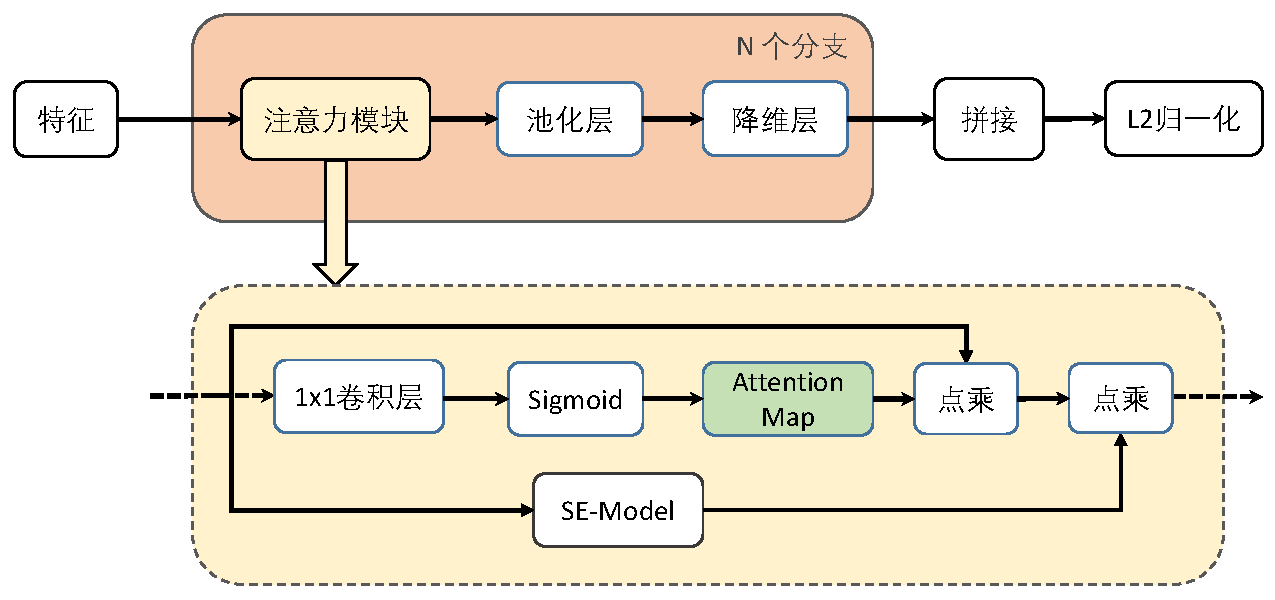
\includegraphics[width=1.0\linewidth]{Img/part.pdf}
  \caption{局部对齐网络的整体架构}
  \label{fig:partnet}
\end{figure}

\subsection{注意力模块}
本小节介绍如图\ref{fig:partnet}中所示的注意力模块。在局部对齐网络中,每一个分支都会生成一个掩膜$M_{i}$,这个掩膜的生成也是局部对齐的关键,其生成过程基于注意力机制,
我们称之为注意力模块。提出的注意力模块包括两个子模块:空间注意力模块和通道注意力模块。空间注意力模块学习空间维度的注意力分布;通道注意力模块则借鉴SE-Net的思想,
认为通道间具有互相依赖的关系,学习通道维度上的权重分布可以有效挖掘这种依赖关系以提升网络表达能力。这两个子模块有着相同的输入,即张量\textbf{T}。
\subsubsection{空间注意力}
对空间注意力的学习旨在挖掘对网络表达能力有益的局部区域特征,根据输入\textbf{T}学习得到一个二维的掩膜$M$并根据$M$更新输入\textbf{T},整个过程分为三个步骤:(1)
使用$1 \times 1$大小的卷积核做\textbf{T}做卷积操作,将\textbf{T}压缩为单通道的特征图。(2)对得到的单通道特征归一化处理,使得所有的特征值分布区间为0到1之间,归一化后
的特征称为注意力分布图(Attention map),即掩膜$M$。Attention map每个值的大小代表着学习到的注意力分布在这个区域的权重大小,特征值越大,注意力权重越大。
(3)将Attention map应用到的输入\textbf{T}之上,完成对空间局部信息的挖掘。

\begin{figure}[h]
  \centering
  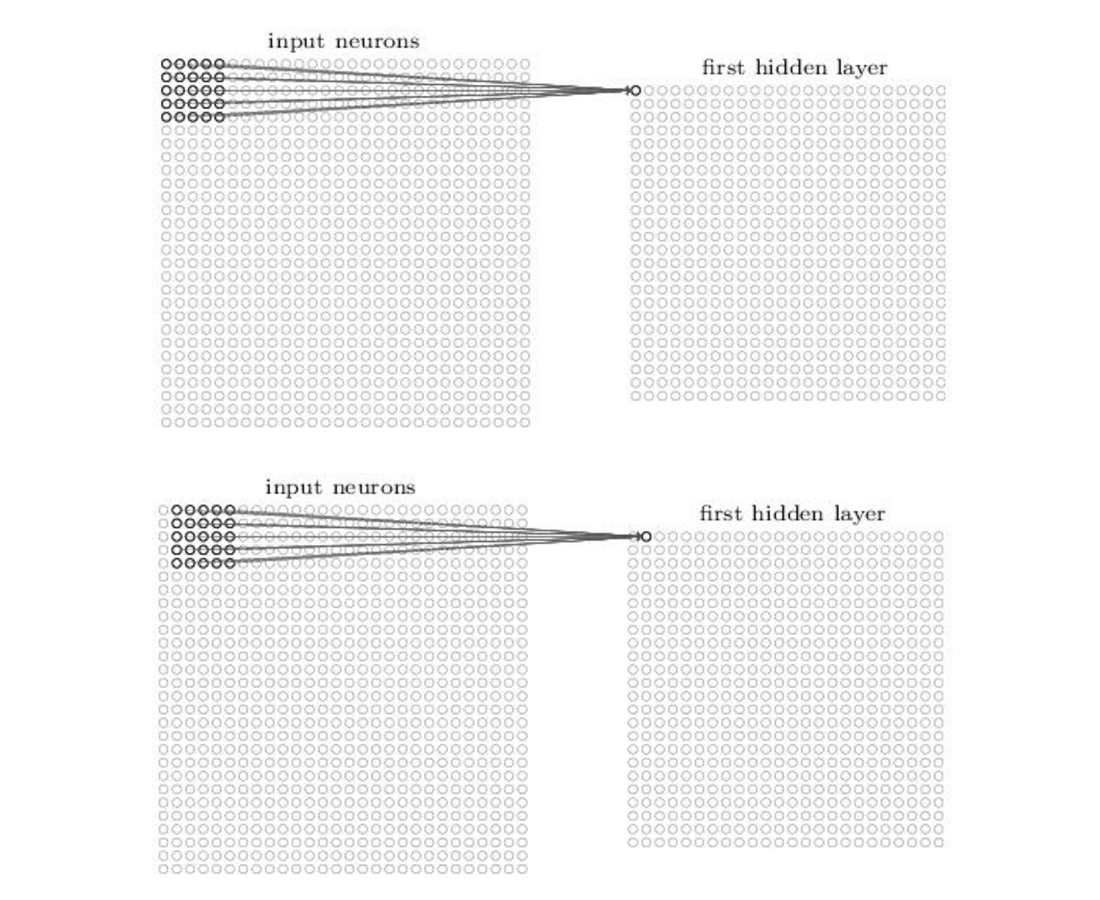
\includegraphics[width=1.0\linewidth]{Img/conv.pdf}
  \caption{对卷积操作的简要说明}
  \label{fig:conv}
\end{figure}

在卷积神经网络出现之前,深度神经网络的每一层网络都和全连接层相连接,下一层的每个输入节点都和当前层的所有输出节点相连接。对于计算机视觉来说,由于其输入是图像,
其空间位置信息对图像的语义理解有着非常重要意义,而全连接层由于和所有输入像素点连接,所以无法捕捉图像的空间信息,这样很不合理。卷积操作是卷积神经网络的核心,如图
\ref{fig:conv}所示,对于一个$28 \times 28$维度的输入,采用$5 \times 5$大小的巻积核通过滑窗的方式逐步计算输出值,这个$5 \times 5$的区域称之为感受野,每次只计算
感受野内部的特征且全局共享这个卷积核的参数,最后得到$24 \times 24$的输出。$5 \times 5$大小的巻积核包含25个权重参数$w$以及一个偏置参数$b$,每次滑窗的计算即卷积核所有权重和对应感受野特征值的相乘
后取和。本方法所提出的空间注意力模块第一步使用的卷积层采用$1 \times 1$大小的卷积核,这个做法的出发点基于$1 \times 1$卷积核的两个特性:(1)进行跨通道的特征交互与整合。
(2)对输入特征的维度变换。Attention map的生成应基于输入\textbf{T},且Attention map的空间维度应与\textbf{T}相同,即$w\times h$。
$1 \times 1$卷积层以\textbf{T}为输入,且与图\ref{fig:conv}中不同的是,卷积的输出可以保留特征的原空间大小,并将$c$个通道压缩至一个。

卷积层输出的特征图在维度上已经和我们需求的Attention map尺度一致,接下来需要对特征值做归一化,保证每个值的大小都在0至1之间,这里我们使用Sigmoid函数去实现归一化,
其表达式为:$\sigma(z)=\frac{1}{1+e^{-z}}$。
一般情况下,Sigmoid在深度神经网络中被用作激活函数,激活函数的意义在于引入非线性,而我们使用Sigmoid的原因在于它的一个重要特性:输出范围为0到1,
如图\ref{fig:sigmoid}所示。由于这个特性的原因,
Sigmoid除了作为激活函数外,也常常被用作二分类的概率输出层,其输出值表示类别为真的概率。在我们提出的注意力模块中,我们可以把Attention map的每个值看作一个二分类的
概率,表示当前区域是否是为需要分配更大权重的局部信息。
\begin{figure}[h]
  \centering
  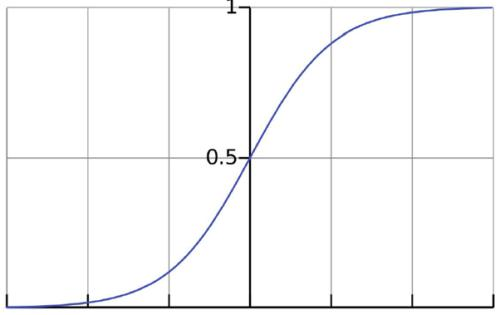
\includegraphics[width=10cm, height=6cm]{Img/sigmoid.jpg}
  \caption{Sigmoid函数}
  \label{fig:sigmoid}
\end{figure}


得到的Attention map为$w\times h$大小的二维特征图,而输入\textbf{T}的为$w\times h \times c$大小的张量,因此需要将Attention map复制$c$份,得到与\textbf{T}相同的尺寸,
两个张量做哈达马积(element-wise product)引入注意力权重,得到空间注意力模块的输出。

\subsubsection{通道注意力}
通道注意力模块借鉴自SE-Net,这个ImageNet 2017 竞赛图像分类的冠军架构在ImageNet 数据集上将 Top-5 error 降低到 2.251\%。近两年来,
SE-Net 因其强大的性能在深度学习领域被广泛使用,也为众多研究人员提供了新的思路和参考。由于SE-Net考虑的是特征图不同通道之间关联性,
所以其初衷并不是为了做视觉注意力,此处视觉注意力特指图像在空间维度的注意力。

Sun等人认为SE-Net通过调节通道间的权重分配也可以强化或者抑制特征图空间区域的局部响应强度,采用多个分支并行的方式,每个分支可以得到不同的局部高响应\cite{sun2018multi}。
这种同构多分支的网络设计方式本质是一种多特征融合,这种策略的有效性也已经在很多任务得到证明:
谷歌于2017年提出的Multi-head attention\cite{vaswani2017attention}将这种结构用于机器翻译任务,使得网络性能得到有效提升;
Hu等人将相同的理念应用在目标检测任务\cite{hu2018relation},也取得了成功。

通道注意力模块单分支的设计与SE-Net一致,如图\ref{fig:partnet}:首先通过全局平均池化(Global average pooling)将输入\textbf{T}压缩$c$维的向量,
然后经过全连接层(FC layer)编码学习通道注意力特征,最后经过Sigmoid归一化。得到的通道注意力向量与空间注意力模块的输出相乘后完成当前分支注意力模块的输出。

\subsection{跨域样本挖掘}
传统的机器学习方法要求源域数据和目标域数据具有相同的分布,从而保证在源域数据集训练的模型性能具有较高的可信度,然而在大多数情况下,训练网络模型的数据集和实际应用场景
之下的数据集很难具有同分布。因此,在已有源域数据训练出的模型的情况下,如何借助模型提取的特征知识,实现模型从源域到相似数据域的迁移具有重大的意义。
本节介绍一种结合在线三元组损失(Online triplet loss),通过已有模型在目标域挖掘无标签样本,并学习其数据分布,达到模型迁移的方法。

\subsubsection{网络训练}
\begin{figure}[h]
  \centering
  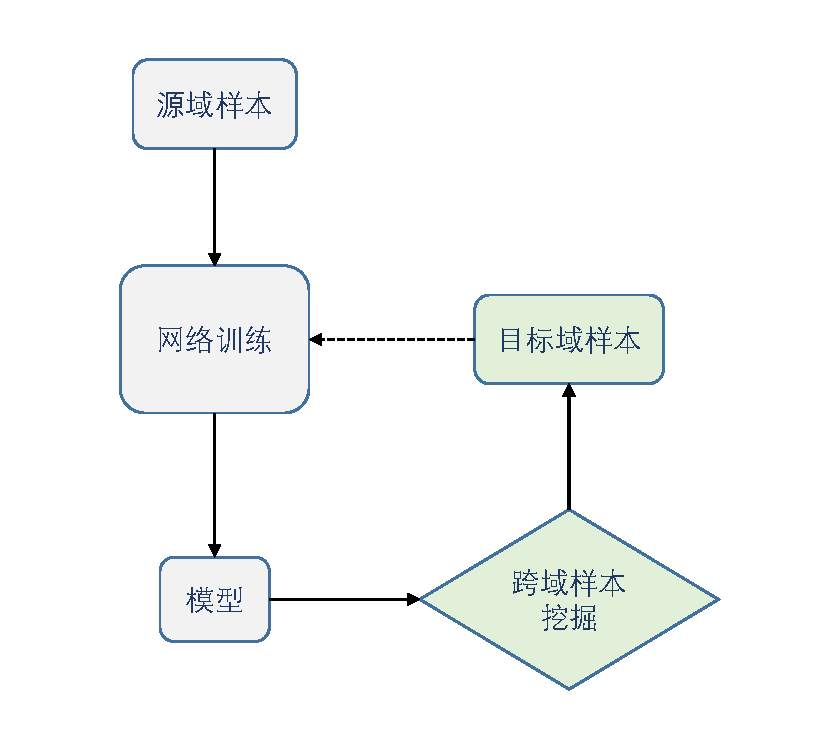
\includegraphics[height=10cm]{Img/crossdomain.pdf}
  \caption{网络训练流程图}
  \label{fig:crossdomain}
\end{figure}

本文所提出的跨域样本挖掘方法是一种可以复用,因此基于此方法的网络训练也是一种迭代的方式,如图\ref{fig:crossdomain}所示,网络的训练流程分为如下步骤:
\begin{itemize}
  \item[1.] 使用源数据域的数据组成训练集,并在此基础上训练出一个模型,训练用的深度网络采用上节所述的局部对齐网络。
  \item[2.] 根据步骤1训练所得模型在目标域做样本挖掘,这一过程会在目标域中获取一定量的样本,并附有标签信息。
  \item[3.] 将在目标域获取的样本和源域样本一起组成新的训练集,重新训练网络,得到新一轮的模型。
  \item[4.] 重复执行步骤2-3多次,直至模型性能稳定。
\end{itemize}

结合企业的实际应用场景来说,用于模型训练的数据一般来自商家拍摄的服装图像,这些数据也就是源域。而模型在实际使用时,输入是用户拍摄的服装图像,
这些由用户拍摄的图像数据集合可以看作是目标域。来自商家的样本一般拍摄质量较高,其中多数为模特摆排,光线等环境条件也比较稳定;而来自用户的检索样本随机性较强,
衣服的形状、摆放位置、光照条件、是否有遮挡或者旋转等因素都十分不稳定。因此,来自商家和来自用户的数据分布具有一定程度的区别。
此外,来自用户上传的检索图像没有标签信息,无法直接用于训练,采用人力标注的方式也不便执行,并且会耗费大量人力资源。

本节提出的跨域样本挖掘的方式可以在目标域挖掘无标签样本,并且可以为其生成伪标签用于网络训练。另外,用户上传的图像数据是一个不断增加的过程,随着目标域数据量的逐步递增
,其数据分布也是一个渐变的过程。基于跨域样本挖掘的网络迭代训练的模式则十分适合这个应用场景,在对过去所学习到的知识的基础上,不断迭代优化以适应新的数据分布,
本质上来说也是一种增量学习。
\subsubsection{样本挖掘}
\begin{figure}[h]
  \centering
  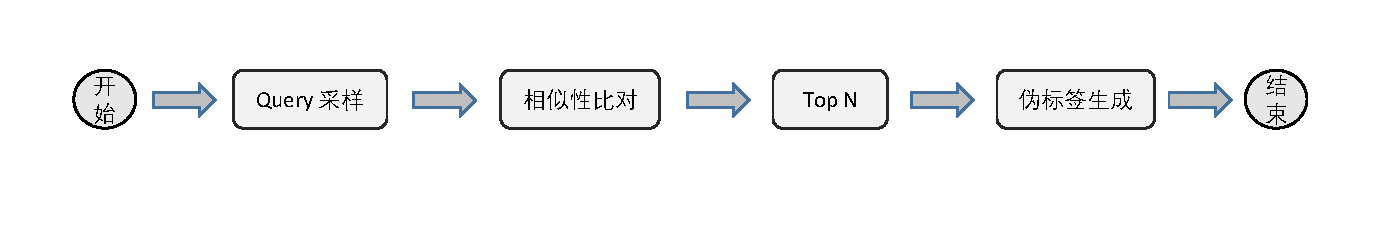
\includegraphics[width=1.0\linewidth]{Img/mining.pdf}
  \caption{样本挖掘流程图}
  \label{fig:mining}
\end{figure}

本小节详细介绍跨域样本挖掘的具体细节,挖掘流程如图\ref{fig:mining}所示:
\begin{itemize}
  \item[1.]Query 采样。我们把模型的输入,即待检索图像称为query,每次基于源域训练集训练得到一个模型之后,从目标域随机采样一部分图像query,剩下的图像作为检索库。
  \item[2.]相似度比对。检索任务的本质是基于相似度或者距离的排序任务,比对的对象是输入的query以及整个检索库里的所有样本。
  以步骤1得到的所有query作为模型的输入,在目标域做检索,根据检索库里图像特征和当前query对应的特征的相似度排序,我们保留top $N$的结果,即前N个和输入query最为相似的图像。
  \item[3.]伪标签生成。对与得到的top $N$的结果,认为前$m$个样本与query是同款服装,前$i$至$j$个样本与query是非同款样本,其中$0<m<i<j<N$。
\end{itemize}
\subsubsection{在线三元组损失}

